\documentclass{article}
\usepackage{graphicx}
\usepackage{epsfig}
%\usepackage{caption}
%\usepackage{subcaption}
\usepackage{epsf}
\usepackage{amssymb}
\usepackage{epstopdf}
\usepackage{amsmath}
\usepackage{braket}
\usepackage{multirow}
\usepackage{array}
\usepackage{mathrsfs}

\makeatletter
\renewcommand{\fnum@figure}{Fig. \thefigure}
\makeatother

\begin{document}

\title{Dipole-Dipole/Cavity-Cavity interaction in the Squeezed Vacuum}
\maketitle 




\section{Three Level Atom}
In this section, we consider a scenario where a three-level atom is located inside the waveguide with the squeezed vacuum injected from both ends, as shown in Fig.~\ref{1}(a). The atomic electronic structure is shown in Fig.~\ref{1}(b) where the atomic states are labeled $|a\rangle$, $|b\rangle$, $|c\rangle$ from the excited state to the ground state. We assume that $\omega_{ac}=2\omega_0$ where $\omega_0$ is the center frequency of the broad band squeed vacuum. $\omega_{ab}$ and $\omega_{bc}$ are not equal but they are still within the bandwith of the squeezed vacuum.  
\begin{figure*}
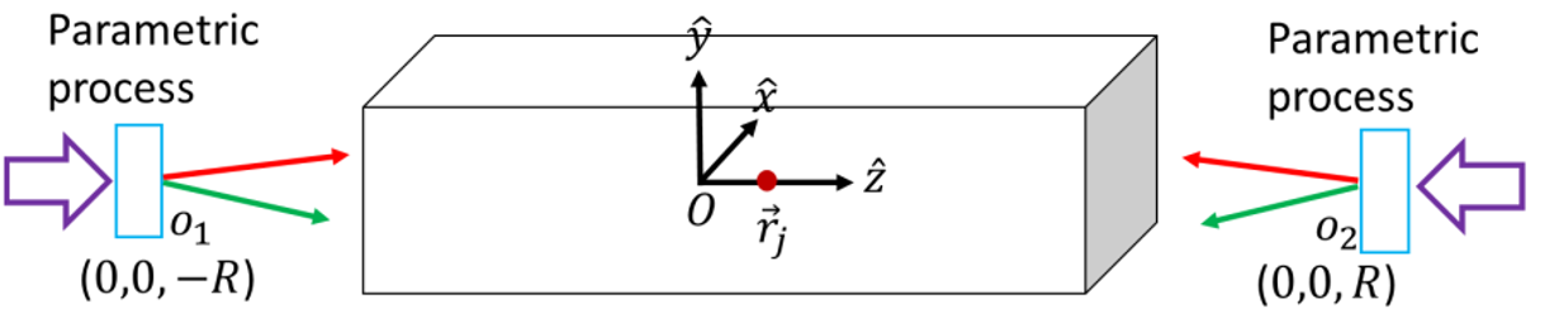
\includegraphics[width=0.7\columnwidth]{fig1.png}
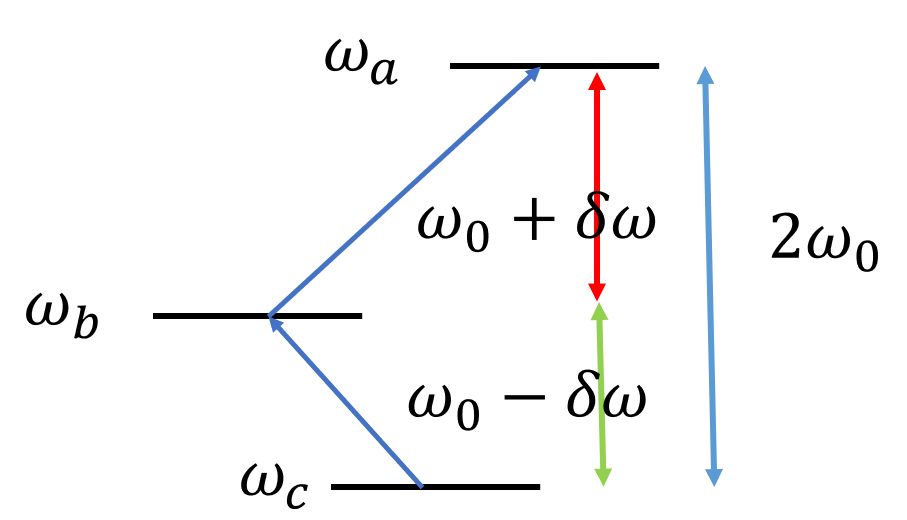
\includegraphics[width=0.25\columnwidth]{fig2.png}
\caption{}
\label{1}
\end{figure*}

The general master equation of dipole-dipole interaction in the squeezed vacuum can be used to study the dynamics of the three-level atom\cite{You2018}:
\begin{equation}
\label{eq1}
\begin{split}
\frac{d\rho^{S}}{dt}=&-i\underset{i\neq j}{\sum}\Lambda_{ij}[S_{i}^{+}S_{j}^{-},\rho^{S}]e^{i(\omega_{i}-\omega_{j})t}\\
&-\frac{1}{2}\underset{i,j}{\sum}\gamma{}_{ij}(1+N)(\rho^{S}S_{i}^{+}S_{j}^{-}+S_{i}^{+}S_{j}^{-}\rho^{S}-2S_{j}^{-}\rho^{S}S_{i}^{+})e^{i(\omega_{i}-\omega_{j})t} \\
&-\frac{1}{2}\underset{i,j}{\sum}\gamma{}_{ij}N(\rho^{S}S_{i}^{-}S_{j}^{+}+S_{i}^{-}S_{j}^{+}\rho^{S}-2S_{j}^{+}\rho^{S}S_{i}^{-})e^{-i(\omega_{i}-\omega_{j})t}\\
&-\frac{1}{2}\sum_{\alpha=\pm}\underset{i,j}{\sum}\gamma'_{ij}Me^{2\alpha ik_{0z}R}e^{i\alpha(\omega_i+\omega_j-2\omega_0)t}(\rho^{S}S_{i}^{\alpha}S_{j}^{\alpha}+S_{i}^{\alpha}S_{j}^{\alpha}\rho^{S}-2S_{j}^{\alpha}\rho^{S}S_{i}^{\alpha})
\end{split}
\end{equation}
where the coefficients are
\begin{equation}
\label{eq2}
\begin{split}
& \gamma_{ij}=\sqrt{\gamma_{i}\gamma_{j}}\cos(k_{0z}r_{ij}) \\
& \Lambda_{ij}=\frac{\sqrt{\gamma_{i}\gamma_{j}}}{2}\sin(k_{0z}r_{ij})\\
& \gamma'_{ij}=\sqrt{\gamma_{i}\gamma_{j}}\cos[k_{0z}(r_{i}+r_{j})]
\end{split}
\end{equation}
where $\gamma_{i}$ is the decay rate for transition $i$ in ordinary vacuum. For a single three level atom, we have $r_i=r_j$, for simplicity we set $R=r_i=0$ and $\gamma_1=\gamma_2=\gamma$. After applying the rotating wave approximation(RWA), the master equation Eq.\eqref{eq1} becomes
\begin{equation}
\label{eq3}
\begin{split}
\frac{d\rho^{S}}{dt}=&-\frac{1}{2}\underset{i}{\sum}\gamma(1+N)(\rho^{S}S_{i}^{+}S_{i}^{-}+S_{i}^{+}S_{i}^{-}\rho^{S}-2S_{i}^{-}\rho^{S}S_{i}^{+})\\
&-\frac{1}{2}\underset{i}{\sum}\gamma N(\rho^{S}S_{i}^{-}S_{i}^{+}+S_{i}^{-}S_{i}^{+}\rho^{S}-2S_{i}^{+}\rho^{S}S_{i}^{-})\\
&-\frac{1}{2}\sum_{\alpha=\pm}\underset{i\ne j}{\sum}\gamma M(\rho^{S}S_{i}^{\alpha}S_{j}^{\alpha}+S_{i}^{\alpha}S_{j}^{\alpha}\rho^{S}-2S_{j}^{\alpha}\rho^{S}S_{i}^{\alpha})
\end{split}
\end{equation}
where $N=\sinh(r)^2$ and $M=\sinh(r)\cosh(r)$The steady state of Eq.\eqref{eq3} can be derived by re-writing Eq.\eqref{eq3} as:
\begin{subequations}
\begin{align}
&\dot{\rho}_{aa}/\gamma=-ch^{2}\rho_{aa}+sh{}^{2}\rho_{bb}-\frac{1}{2}chsh(\rho_{ac}+\rho_{ca})\label{4a} \\
& \dot{\rho}_{bb}/\gamma=(ch^{2}\rho_{aa}-sh^{2}\rho_{bb})+(sh^{2}\rho_{cc}-ch^{2}\rho_{bb})+chsh(\rho_{ac}+\rho_{ca})\label{4b}\\
&\dot{\rho}_{cc}/\gamma=ch^{2}\rho_{bb}-sh^{2}\rho_{cc}-\frac{1}{2}chsh(\rho_{ac}+\rho_{ca})\label{4c}\\
&(\dot{\rho}_{ac}+\dot{\rho}_{ca})/\gamma=-\frac{1}{2}(ch^{2}+sh^{2})(\rho_{ac}+\rho_{ca})-shch(\rho_{aa}-2\rho_{bb}+\rho_{cc})\label{4d}\\
&\dot{\rho}_{ab}/\gamma=-(1+\frac{3}{2}sh^{2})\rho_{ab}-\frac{1}{2}chsh\rho_{cb}\label{4e}\\
&\dot{\rho}_{cb}/\gamma=-\frac{1}{2}chsh\rho_{ab}-(\frac{1}{2}+\frac{3}{2}sh^{2})\rho_{cb}\label{4f}
\end{align}
\end{subequations}
where $sh=\sinh(r), ch=\cosh(r)$. Eq.\eqref{4e}\eqref{4f} yield $\rho_{ab}=\rho_{cb}=0$ for the steady state, and Eq.\eqref{4a}-\eqref{4d} yield $\rho_{aa}=\frac{sh^{2}}{sh^{2}+ch^{2}}$, $\rho_{cc}=\frac{ch^{2}}{sh^{2}+ch^{2}}$, $\rho_{ac}=-\frac{shch}{sh^{2}+ch^{2}}$. Thus, the steady state is actually a superposition state of $|a\rangle$ and $|c\rangle$: $\frac{sh}{\sqrt{sh^{2}+ch^{2}}}|a\rangle-\frac{ch}{\sqrt{sh^{2}+ch^{2}}}|c\rangle$. This phenomenon is similar to coherent trapping, but here we achieve the trapping for $\Xi$ structure with the squeezed vacuum reservoir, which cannot be realized with coherent pump due to spontaneous emission.
%\begin{equation}
%\label{eq4}
%\begin{split}
%\frac{d\rho^{S}}{dt}=&\sum_{i\ne j}\frac{\gamma}{2}[-\rho(\cosh rS_{i}^{\dagger}+\sinh rS_{j})(\cosh rS_{i}+\sinh rS_{j}^{\dagger})\\
%&-(\cosh rS_{i}^{\dagger}+\sinh rS_{j})(\cosh rS_{i}+\sinh rS_{j}^{\dagger})\rho\\
%&+2(\cosh rS_{i}+\sinh rS_{j}^{\dagger})\rho(\cosh rS_{i}^{\dagger}+\sinh rS_{j})]
%\end{split}
%\end{equation}


\section{Cavity-Cavity interaction}
In this section, we consider a similar scenario but now the atoms are replaced with single mode cavity. The total Hamiltonian is:
\begin{equation}
\label{eq5}
\begin{split}
H=\sum_{i}\hbar\omega(a^{\dagger}a_{i}+\frac{1}{2})+\hbar\sum_{i,k}\omega_{k}(a_{i}^{\dagger}a_{i}+\frac{1}{2})+\hbar\sum_{i,k}g_{k}(a_{i}^{\dagger}a_{k}+H.c.)
\end{split}
\end{equation}
where $a_k$ stands for the mods in the waveguide and $a$ is the field operator of the single mode inside the cavity. The waveguide is saturated with the squeezed vacuum with the center frequency $\omega_0$. 

First, we study two non-resonant cavities coupled to the squeezed vacuum reservoir. The eigen frequencies of these two cavities are $\omega_1=\omega_0-\delta \omega$ and $\omega_2=\omega_0+\delta \omega$, following exacly the same steps as the derivation of Eq.\eqref{eq1}, we get:
\begin{equation}
\label{eq6}
\begin{split}
\dot{\rho}&=\sum_{i}\gamma(1+N)(-\rho a_{i}^{\dagger}a_{i}-a_{i}^{\dagger}a_{i}\rho+2a_{i}\rho a_{i}^{\dagger})\\
&+\gamma N(-\rho a_{i}a_{i}^{\dagger}-a_{i}a_{i}^{\dagger}\rho+2a_{i}^{\dagger}\rho a_{i})\\
&+\sum_{i\ne j}\gamma M(e^{i(\theta_i+\theta_j)}\rho a_{i}a_{j}+e^{i(\theta_i+\theta_j)}a_{i}a_{j}\rho-2e^{i(\theta_i+\theta_j)}a_{i}\rho a_{j}+h.c.)\\
\end{split}
\end{equation}
where $\theta_i$ is a phase factor which depends on the relative position of cavities and the squeezing source. The above equation can be re-arranged as:
\begin{equation}
\label{eq7}
\begin{split}
\dot{\rho}&=\sum_{i\ne j}\frac{\gamma}{2}[-\rho(\cosh ra_{i}^{\dagger}-e^{i\theta}\sinh ra_{j})(\cosh ra_{i}-e^{-i\theta}\sinh ra_{j}^{\dagger})\\
&-(\cosh ra_{i}^{\dagger}-e^{i\theta}\sinh ra_{j})(\cosh ra_{i}-e^{-i\theta}\sinh ra_{j}^{\dagger})\rho\\
&+2(\cosh ra_{i}-e^{-i\theta}\sinh ra_{j}^{\dagger})\rho(\cosh ra_{i}^{\dagger}-e^{i\theta}\sinh ra_{j})]\\
\end{split}
\end{equation}
we use the following Bogoliubov transformation\cite{Bogoliubov}:
\begin{equation}
\label{eq8}
\begin{split}
&S=exp(\eta^{\star}a_{i}a_{j}-\eta a_{i}^{\dagger}a_{j}^{\dagger})\\
&A_{i}=S^{+}a_{i}S=\cosh(r)a_{i}-e^{-i\theta}\sinh(r)a_{j}^{\dagger} \\
&A_{i}^{+}=S^{+}a_{i}^{+}S=\cosh(r)a_{i}^{+}-e^{i\theta}\sinh(r)a_{j}\\
\end{split}
\end{equation}
so the master equation Eq.\eqref{eq7} becomes:
\begin{equation}
\label{eq9}
\begin{split}
\dot{\rho}=\sum_{i}\gamma[-\rho A_{i}^{\dagger}A_{i}-A_{i}^{\dagger}A_{i}\rho+2A_{i}\rho A_{i}^{\dagger}]
\end{split}
\end{equation}
Next we redefine the density matrix: $\rho_{s}=S\rho S^{\dagger}$. Thus Eq.\eqref{eq9} becomes:
\begin{equation}
\label{eq11}
\begin{split}
\dot{\rho}_{s}&=\sum_{i}\gamma[-\rho_{s}a_{i}^{\dagger}a_{i}-a_{i}^{\dagger}a_{i}\rho_{s}+2a_{i}\rho_{s}a_{i}^{\dagger}]\\
&\equiv\sum_{i}\gamma[-a_{i}^{l\dagger}a_{i}^{l}\rho_{s}-a_{i}^{r\dagger}a_{i}^{r}\rho_{s}+2a_{i}^{r}a_{i}^{l\dagger}\rho_{s}]\equiv L\rho_{s}
\end{split}
\end{equation}
Here we define superoperator $\{a_{i}^{l}, a_{i}^{l\dagger}\}$($\{a_{i}^{r}, a_{r}^{l\dagger}\}$ ) only acting to the left(right) on density operator $\rho$ \cite{Wang2002, An}. These operators have the following commutation relations: 
\begin{equation}
\label{eq12}
\begin{split}
[a_{i}^{r},a_{j}^{r\dagger}]=\delta_{ij},\,[a_{i}^{l},a_{j}^{l\dagger}]=-\delta_{ij},\,[a_{i}^{l},a_{j}^{r\dagger}]=[a_{i}^{l},a_{j}^{r}]=[a_{i}^{l\dagger},a_{j}^{r}]=[a_{i}^{l\dagger},a_{j}^{r\dagger}]=0
\end{split}
\end{equation}
Thus, the steady state of Eq.\eqref{eq11} can be solved by solving $L\rho=0$, which requires the diagnolization of superoperator $L$. Applying the similarity transformation $U=e^{-a_{1}^{r}a_{1}^{l\dagger}-a_{2}^{r}a_{2}^{l\dagger}}$ to Eq.\eqref{eq11} , since we have $U^{-1}(a_{i}^{r\dagger},a_{i}^{l},a_{i}^{r},a_{i}^{l\dagger})U=(a_{i}^{r\dagger}+a_{i}^{l\dagger},a_{i}^{r}+a_{i}^{l},a_{i}^{r},a_{i}^{l\dagger})$, the right hand side of Eq.\eqref{eq11} becomes:
\begin{equation}
\label{eq13}
\begin{split}
RHS=\sum_{i}\gamma U^{-1}[-a_{i}^{l\dagger}a_{i}^{l}-a_{i}^{r\dagger}a_{i}^{r}+2a_{i}^{r}a_{i}^{l\dagger}]UU^{-1}\rho_{s}=\sum_{i}\gamma[-a_{i}^{l\dagger}a_{i}^{l}-a_{i}^{r\dagger}a_{i}^{r}]U^{-1}\rho_{s}
\end{split}
\end{equation}
The only solution to $L\rho=0$ is $U^{-1}\rho_{s}=|0,0\rangle\langle0,0|$, which yields $\rho=S^{\dagger}\rho_S S=S^{\dagger}e^{-K_{-1}-K_{-2}}|0,0\rangle\langle0,0|S=S^{\dagger}|0,0\rangle\langle0,0|S$ which is the two mode squeezed vacuum.

Then we study the case where two cavities are identical, i.e., $\omega_1=\omega_2=\omega_0$. Then the master equation becomes:
\begin{equation}
\label{eq13}
\begin{split}
\dot{\rho}&=\sum_{ij}\gamma\cosh^{2}r(-\rho a_{i}^{\dagger}a_{j}-a_{i}^{\dagger}a_{j}\rho+2a_{i}\rho a_{j}^{\dagger})\\
&+\gamma\sinh^{2}r(-\rho a_{i}a_{j}^{\dagger}-a_{i}a_{j}^{\dagger}\rho+2a_{i}^{\dagger}\rho a_{j})\\
&+\gamma\cosh r\sinh r(e^{i(\theta_{i}+\theta_{j})}\rho a_{i}a_{j}+e^{i\theta}a_{i}a_{j}\rho-e^{i\theta}2a_{i}\rho a_{j}+h.c.)\\
\end{split}
\end{equation}
This equation can be rearranged when $\theta_1=\theta_2=\theta$:
\begin{equation}
\label{eq14}
\begin{split}
\dot{\rho}&=\sum_{ij}\gamma[-\rho(\cosh ra_{i}^{\dagger}-e^{i\theta}\sinh ra_{i})(\cosh ra_{j}-e^{-i\theta}\sinh ra_{j}^{\dagger})\\
&-(\cosh ra_{i}^{\dagger}-e^{i\theta}\sinh ra_{i})(\cosh ra_{j}-e^{-i\theta}\sinh ra_{j}^{\dagger})\rho\\
&+2(\cosh ra_{j}-e^{-i\theta}\sinh ra_{j}^{\dagger})\rho(\cosh ra_{i}^{\dagger}-e^{i\theta}\sinh ra_{i})]\\
\end{split}
\end{equation}
We introduce the Bogoliubov transformation:
\begin{equation}
\label{eq15}
\begin{split}
&S_{i}=exp(\eta^{\star}a_{i}^{2}-\eta a_{i}^{\dagger2})\\
&A_{i}=S_{i}^{+}a_{i}S_{i}=\cosh(r)a_{i}-e^{-i\theta}\sinh(r)a_{i}^{\dagger} \\
&A_{i}^{+}=S_{i}^{+}a_{i}^{+}S_{i}=\cosh(r)a_{i}^{+}-e^{i\theta}\sinh(r)a_{i}\\
\end{split}
\end{equation}
so master equation Eq.\eqref{eq14} becomes
\begin{equation}
\label{eq16}
\begin{split}
\dot{\rho}=\sum_{ij}\gamma[-\rho A_{i}^{\dagger}A_{j}-A_{i}^{\dagger}A_{j}\rho+2A_{j}\rho A_{i}^{\dagger}]
\end{split}
\end{equation}
Next we define $ \rho_{s}=S_{1}S_{2}\dot{\rho S_{1}^{+}S_{2}^{+}}$ so the master equation is reduced to:
\begin{equation}
\label{eq17}
\begin{split}
\dot{\rho_{s}}=\sum_{ij}\gamma[-\rho_{s}a_{i}^{\dagger}a_{j}-a_{i}^{\dagger}a_{j}\rho_{s}+2a_{j}\rho_{s}a_{i}^{\dagger}]
\end{split}
\end{equation}
To diagnolize this Lindblad equation, we introduce the transformation: $$\begin{array}{c}
L_{1}\\
L_{2}
\end{array}=\begin{array}{c}
\frac{1}{\sqrt{2}}(a_{1}-a_{2})\\
\frac{1}{\sqrt{2}}(a_{1}+a_{2})
\end{array}$$
where $[L_{i},L_{j}^{\dagger}]=\delta_{ij}$, and the master equation becomes:
\begin{equation}
\label{eq18}
\begin{split}
\dot{\rho_{s}}&=\gamma[-2\rho_{s}L_{2}^{\dagger}L_{2}-2L_{2}^{\dagger}L_{2}\rho_{s}+4L_{2}\rho_{s}L_{2}^{\dagger}]\\
&=\gamma[-2L_{2}^{r\dagger}L_{2}^{r}\rho_{s}-2L_{2}^{l\dagger}L_{2}^{l}\rho_{s}+4L_{2}^{l}L_{2}^{r\dagger}\rho_{s}]\\
&=L\rho
\end{split}
\end{equation}
Operator $L_2^{\dagger}$ has the following properties: $$L_{2}^{\dagger}|0\rangle=\frac{1}{\sqrt{2}}(|01\rangle+|10\rangle)\equiv|1_{L}\rangle$$ $$L_{2}^{\dagger}\frac{1}{\sqrt{2}}(|01\rangle+|10\rangle)=\sqrt{2}[\frac{1}{2}(|02\rangle+\sqrt{2}|11\rangle+|20\rangle)]=\sqrt{2}|2_{L}\rangle$$  $$L_{2}^{\dagger}\frac{1}{2}(|02\rangle+\sqrt{2}|11\rangle+|20\rangle)=\sqrt{3}[\frac{1}{2\sqrt{2}}(|03\rangle+\sqrt{3}|12\rangle+\sqrt{3}|21\rangle+|30\rangle)]=\sqrt{3}|3_{L}\rangle$$  $$...$$
Then we use the similarity transformation: $e^{-L^{r}L^{l\dagger}}$, which yields $U^{-1}(L_{2}^{r\dagger},L_{2}^{l},L_{2}^{l\dagger},L_{2}^{r})U=(L_{2}^{r\dagger}+L_{2}^{l\dagger},L_{2}^{l}+L_{2}^{r},L_{2}^{l\dagger},L_{2}^{r}) $. Thus, the master equation Eq.\eqref{eq18} becomes:
\begin{equation}
\label{eq18}
\begin{split}
RHS=\gamma U^{-1}[-L_2^{l\dagger}L_2^{l}-L_2^{r\dagger}L_2^{r}+2L_2^{r}L_2^{l\dagger}]UU^{-1}\rho_{s}=\gamma[-L_2^{l\dagger}L_2^{l}-L_2^{r\dagger}L_2^{r}]U^{-1}\rho_{s}
\end{split}
\end{equation}
The only solution to the steady state is $\rho_{s}=e^{-L^{r}L^{l\dagger}}|0_{L}\rangle\langle0_{L}|=|0\rangle\langle0|$ which yields $\rho=S_{1}^{+}S_{2}^{+}|0\rangle\langle0|S_{1}S_{2}$. Thus, when there are more than one cavities, as long as they are all resonant to the center frequency of the broadband squeezed vacuum, the cavity fields' steady states are single mode squeezed vacuum as if there is no interaction at all.


\begin{thebibliography}{99}
\bibitem{You2018} Jieyu You, Zeyang Liao, Sheng-Wen Li, and M. Suhail Zubairy, Phys. Rev. A 97, 023810 
\bibitem{Bogoliubov} Bogolubov N N 1947 J. Phys. (USSR) 11 23
\bibitem{Wang2002} Wang S J et al. 2002 Phys. Rev. A 66 033608(2002)
\bibitem{An} Jun-Hong An, Shun-Jin Wang, Hong-Gang Luo, Cheng-Long Jia Chin. Phys. Lett., Vol 21, No. 1
\end{thebibliography} 
\end{document}